\chapter{Evaluation}\label{chap:evaluation}
We put the performance of all the parallel merge implementations 
on Titan-Z in Chapter \ref{chap:implementation} in Figure \ref{fig:titan-z}.
\begin{figure}[!bh]
\begin{center}
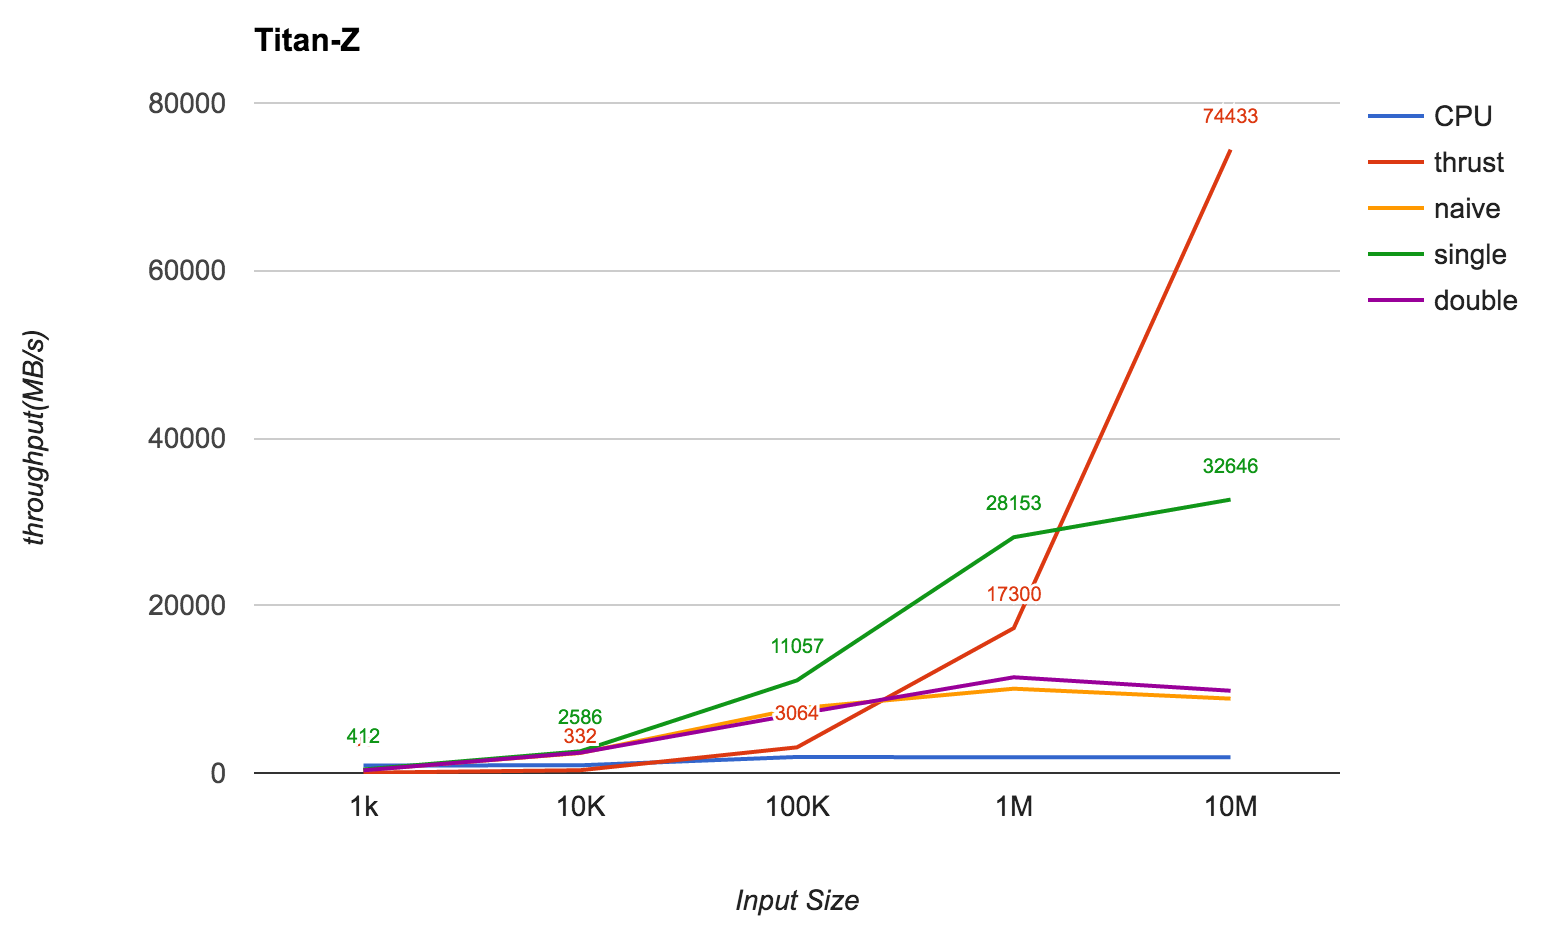
\includegraphics[width=\textwidth]{titan-z.png}
\end{center}
\caption{{\label{fig:titan-z}} Performance on Titan-Z}
\end{figure}

Among the three implementations we have, single buffer parallel merge has the 
best performance. Compared to thrust merge implementation, single buffer 
parallel merge can achieve up to 3x speedup for input size between 10k to 1M.

We also test the portability of our implementations on an Nvidia GTX980 GPU (Maxwell 
Architecture). Figure \ref{fig:maxwell} shows the performance.
\begin{figure}[!bh]
\begin{center}
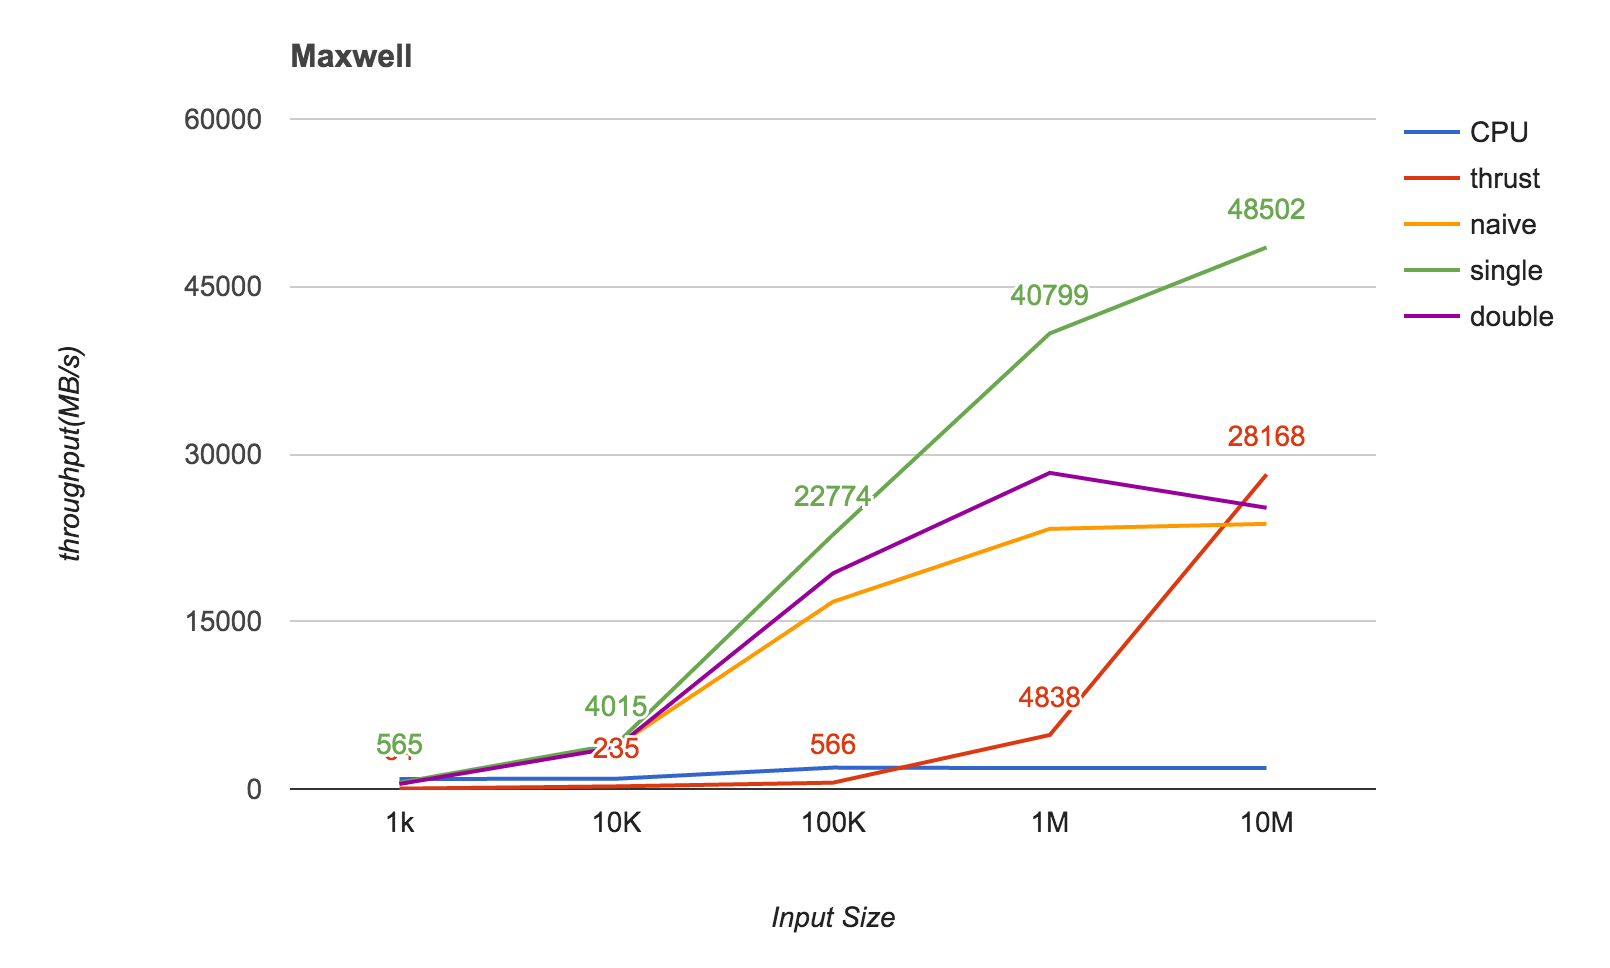
\includegraphics[width=\textwidth]{maxwell.png}
\end{center}
\caption{{\label{fig:maxwell}} Performance on GTX980}
\end{figure}

Single buffer parallel merge outperforms the other two implementations as well.
Compared to thrust merge, single buffer parallel merge can achieve up to 20x 
speedup. The reason is that thrust merge is not specifically optimized for 
Maxwell Architecture and therefore its performance is far from optimal on this 
architecture. 
